205. \begin{figure}[ht!]
\center{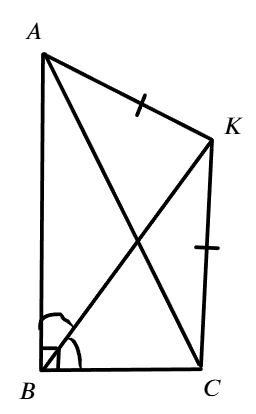
\includegraphics[scale=0.35]{g9-203.png}}
\end{figure}\\
Так как $BK$ является биссектрисой, $\angle ABK=\angle KBC=90^\circ:2=45^\circ.$ Пусть $BC=3x,$ тогда $AB=4x$ и по теореме косинусов для треугольника $AKB$ имеет место соотношение $AK^2=16x^2+\cfrac{49}{2}-2\cdot\cfrac{7}{\sqrt{2}}\cdot 4x\cdot \cfrac{\sqrt{2}}{2},\ AK^2=16x^2+\cfrac{49}{2}-28x.$ По теореме косинусов для треугольника $KBC$ имеет место равенство $KC^2=9x^2+\cfrac{49}{2}-2\cdot 3x\cdot\cfrac{7}{\sqrt{2}}\cdot \cfrac{\sqrt{2}}{2},\ KC^2=9x^2+\cfrac{49}{2}-21x.$ Так как $AK=KC,$ получим равенство $16x^2+\cfrac{49}{2}-28x=9x^2+\cfrac{49}{2}-21x,\ 7x^2=7x,\ x=1.$ Тогда $DK=\sqrt{9x^2+16x^2}=\sqrt{25x^2}=\sqrt{25}=5.$\\
